\Chapter{Modelo de reconhecimento de gestos}

Neste trabalho, formula-se um modelo de reconhecimento de gestos do corpo para
controle de um avatar animado em um ambiente virtual. Nesse ambiente um personagem que representa o usuário, aguarda que um gesto seja reconhecido para que ele possa executar a animação correspondente.

Para este propósito, cinco gestos foram estabelecidos: andar para direita, andar para esquerda, levantar o braço direito, levantar o braço esquerdo e levantar ambos os braços.

O modelo proposto está estruturado em cinco módulos: a captura e segmentação das imagens, a extração de características e quantização vetorial, a criação e treinamento das HMMs, a identificação das sequências de símbolos e o ambiente virtual. A Figura \ref{img:diagrama_do_sistema} exibe um diagrama do modelo proposto.

\begin{figure}[!htbp]
  \center
  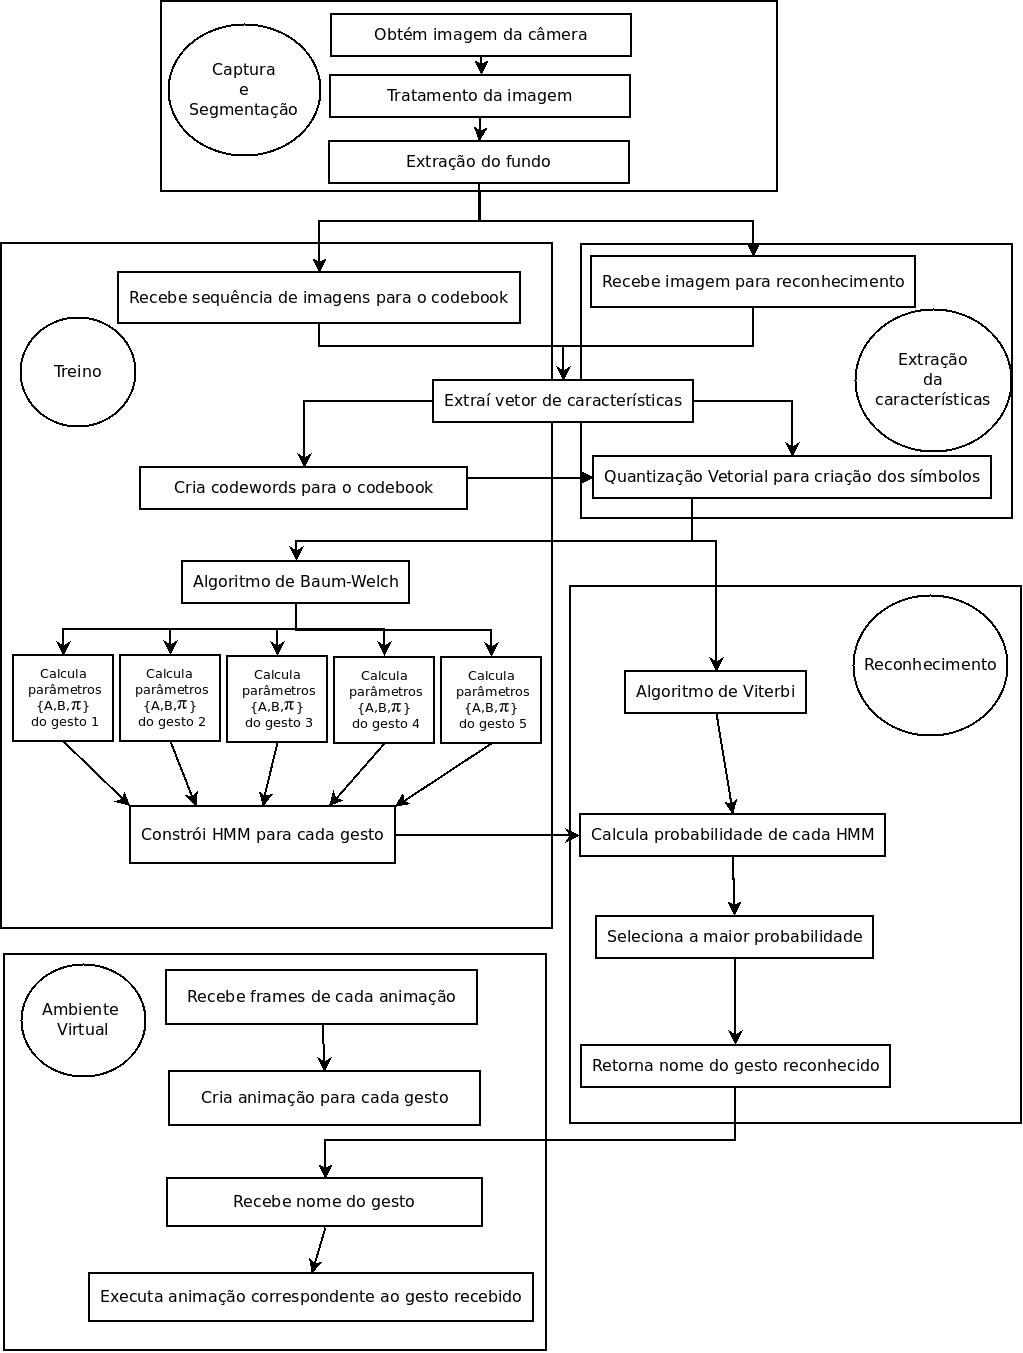
\includegraphics[scale=0.40]{imagens/diagrama_do_sistema.jpg}
  \caption{Diagrama geral do sistema.}
  \label{img:diagrama_do_sistema}
\end{figure}

No processo de captura e segmentação, foi utilizada a biblioteca OpenCV\footnote{OpenCV (Open Source Computer Vision) - http://opencv.willowgarage.com/wiki} , para obtenção de imagens a partir de uma webcam e para processamento dessas imagens com o objetivo de obter imagens binárias, neste caso com o fundo em cor preta e o usuário detectado em cor branca. Os frames \(F_i\) capturados possuem altura \(A_f\) de tamanho 640 pixels e largura \(L_f\) de 480 pixels e foram capturadas a uma taxa de 30 fps(frames por segundo).

Para que as sequências de frames possam ser aplicadas a HMMs, elas precisam ser transformadas em sequências de símbolos \(S\), portanto as imagens segmentadas são enviadas para o módulo que extrairá delas padrões de interesse segundo um algoritmo de reconhecimento de padrões, nesse caso usamos quantização vetorial, como é normalmente usado em HMMs. O espaço de características é dividido em clusters, codewords que representam os centros desses clusters são necessárias, o índice da codeword \(C_f\) é atribuído ao símbolo \(S_f\).

As características obtidas formam o vetor de características daquele frame \(V_f\). Esse vetor de características é enviado para o módulo de quantização vetorial, que retorna o índice que será usado como símbolo do grupo ao qual esse vetor foi agrupado. Para esse processo, foi utilizada a biblioteca SciPy\footnote{SciPy (Scientific Tools for Python) - http://www.scipy.org}.

No processo de modelagem, treinamento e identificação dos gestos foram utilizadas HMMs. A biblioteca GHMM\footnote{GHMM (General Hidden Markov Model library) - http://ghmm.org} foi utilizada para esse propósito.

De cada gesto foram gravados cinco vídeos, executando os gestos de forma um pouco diferente, quatro desses vídeos foram usados para o treinamento de suas respectivas HMMs, esse treino foi feito utilizando-se os valores dos índices retornados pela quantização vetorial do vetor de características de cada frame desses vídeos. O quinto vídeo foi gravado com o propósito de testar os modelos.

Durante a execução em tempo real de identificação dos gestos, a cada segundo de vídeo, uma sequência de índices é avaliada em cada um dos cinco modelos ocultos de Markov e a probabilidade dessa sequência pertencer ao modelo é armazenada. O gesto reconhecido será aquele representado pelo modelo que retornou a probabilidade mais alta.

O gesto identificado ativa uma função que executa a animação correspondente do avatar no ambiente virtual, dentro de um conjunto de animações possíveis previamente criadas.

\section{Captura e segmentação}

No processo de captura, as imagens são capturas em uma taxa de 30 frames por segundo, através da biblioteca OpenCV. OpenCV é uma biblioteca de visão computacional, escrita em C e C++ e roda em Linux, Windows e Mac OS X. Com interface para linguagens como Python, Ruby, Matlab e outras. OpenCV foi projetada para eficiência e aplicativos em tempo real, usar vantagens de processadores com vários núcleos. A biblioteca contém mais de 500 funções que se espalham por várias áreas de visão computacional,
além de módulos de processamento de imagem e vídeo I/O, estrutura de dados, álgebra linear,
GUI (Inteface Gráfica do Usuário) básica com sistema de janelas independentes, controle de
mouse e teclado, calibração de câmera, reconhecimento de objetos e análise estrutural e
é um software aberto ao uso acadêmico e comercial \cite{LearningOpenCV}.

As imagens são pré-processadas com as funções de OpenCV para poder, finalmente, ter características extraídas.

\subsection{Extração do fundo}

No início do módulo de captura, é necessário que o sistema armazene uma imagem do fundo do ambiente, ela será utilizada durante o processo de extração do fundo.

Todos os frames seguintes sofrem uma operação de subtração em relação ao frame de fundo.
A imagem resultante passará por um processo de binarização segundo uma tolerância, que dita a partir de quanta diferença os pixels devem ser considerados brancos, todos os pixels que ficarem abaixo dessa diferença serão pretos. A Figura \ref{img:processo_segmentacao} demonstra um exemplo de processo de  subtração de fundo do sistema.

\begin{figure}[!htbp]
\center
\subfigure[img:fundo][Fundo]{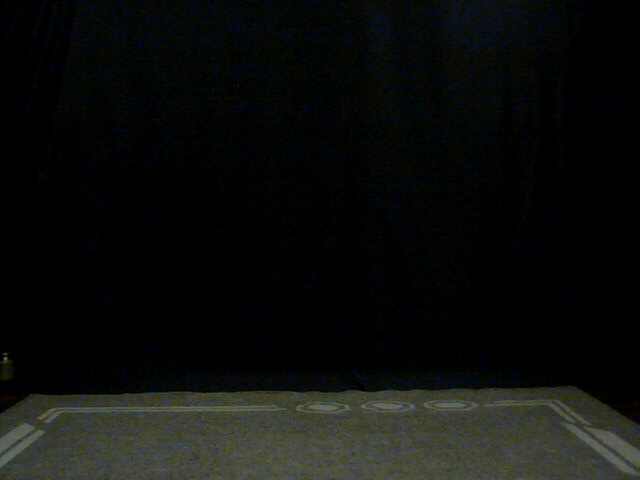
\includegraphics[width=5cm]{imagens/fundo.jpg}}
\qquad
\subfigure[img:frame][Imagem]{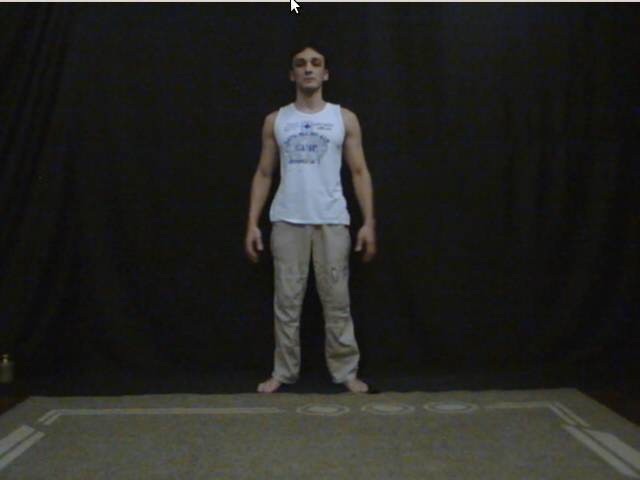
\includegraphics[width=5cm]{imagens/frame.jpg}}
\qquad
\subfigure[img:mascara][Subtração]{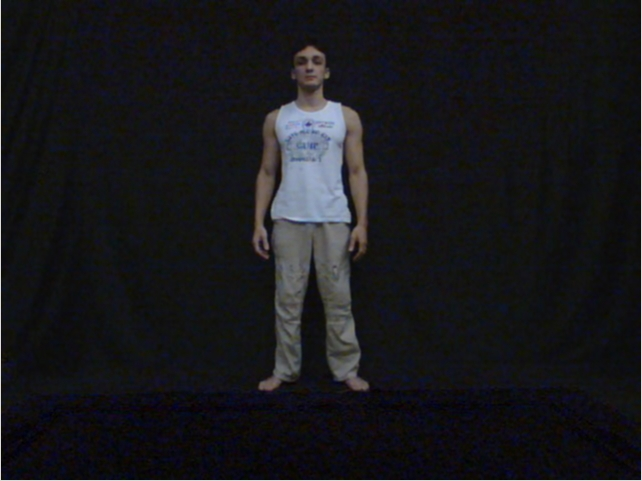
\includegraphics[width=5cm]{imagens/mascara.jpg}}
\qquad
\subfigure[img:binario][Binário]{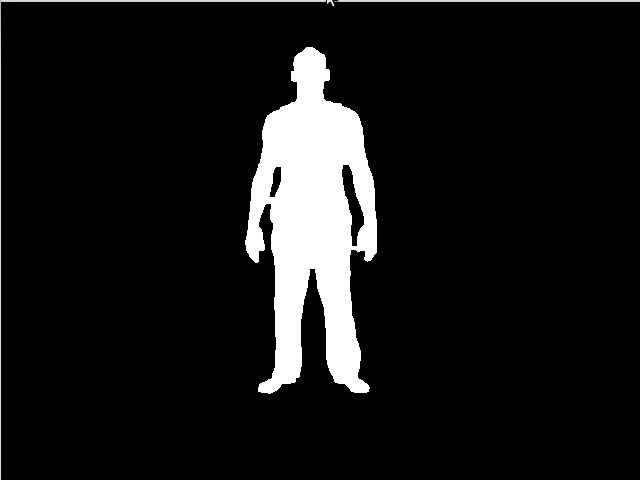
\includegraphics[width=5cm]{imagens/binario.jpg}}
\caption{Processo de segmentação}
\label{img:processo_segmentacao}
\end{figure}



\subsection{Processamento das imagens}

É importante realizar alguns pré-processamentos e pós-processamentos nas imagens com o intuito de melhorar a silhueta detectada e remover ruídos e informações desnecessárias. Esses processamentos são operações morfológicas, suavização e eliminação de falsas detecções.

\subsubsection{A) Remoção de ruídos}

Todos os frames capturados, inclusive a imagem de fundo, são tratados com filtro de gauss com objetivo de suavizar as imagens, removendo assim, ruídos da imagem antes de sofrerem o processo de subtração, a Figura \ref{img:gauss_process} demonstra o efeito do filtro de Gauss com kernel de tamanho $3\times3$ no processo de eliminação de pequenos ruídos, esses efeitos não ficaram tão evidentes porque nos ambientes onde as gravações foram feitas havia condições ideais de iluminação, a câmera estava adequadamente configurada e o fundo era completamente estático e simples.

\begin{figure}[!htbp]
\subfigure[img:arms_up][Imagem]{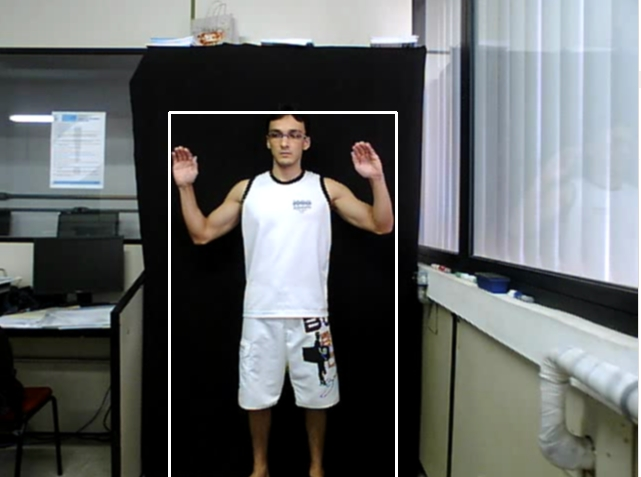
\includegraphics[width=5cm]{imagens/arms_up.jpg}}
\subfigure[img:no_gauss][Antes do filtro]{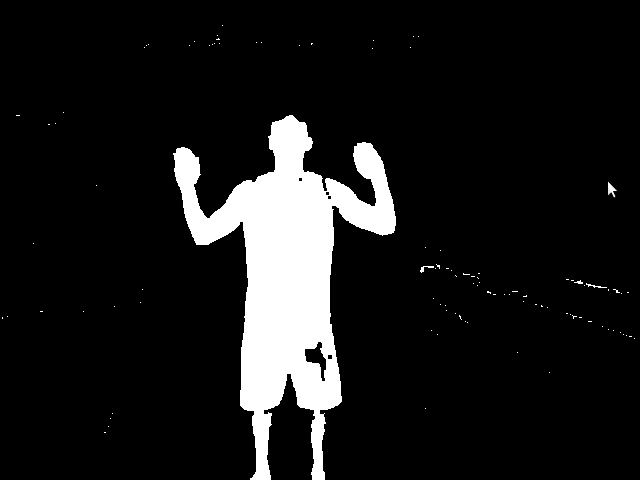
\includegraphics[width=5cm]{imagens/no_gauss.jpg}}
\subfigure[img:gauss][Após o filtro]{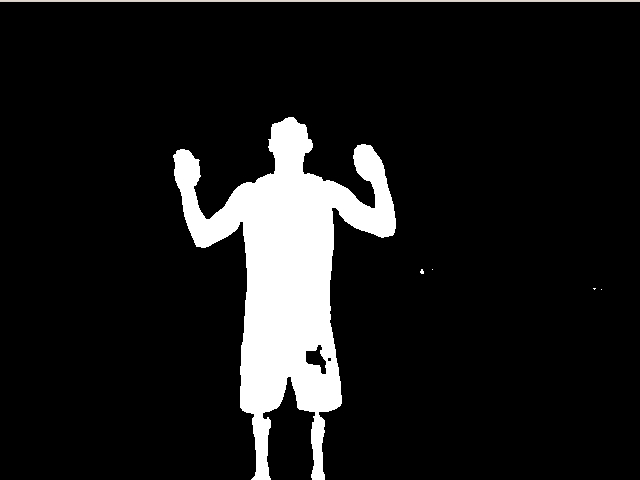
\includegraphics[width=5cm]{imagens/gauss.jpg}}
\caption{Pequenos ruídos sendo eliminados pelo filtro de Gauss}
\label{img:gauss_process}
\end{figure}

\subsubsection{B) Operações morfológicas}

Um filtro de dilatação (\textit{dilate}), que expande os pixels na imagem, foi aplicado na imagem binária, com a intenção de remover falhas no interior da silhueta, em conjunto com um filtro de erosão (\textit{erode}), em seguida, para transformar a silhueta dilatada, mas sem essas falhas, na silhueta com tamanho normal. Através da Figura \ref{img:dilate_erode} é possível observar pequenos espaços dentro da silhueta sendo conectados pelo processo de dilatação e gerando uma silhueta maior do que a primeira e esse efeito sendo atenuado pelo filtro de erosão. O resultado é uma silhueta próxima a original, mas sem as falhas internas.

\begin{figure}[!htbp]
\subfigure[img:arms_up][Imagem]{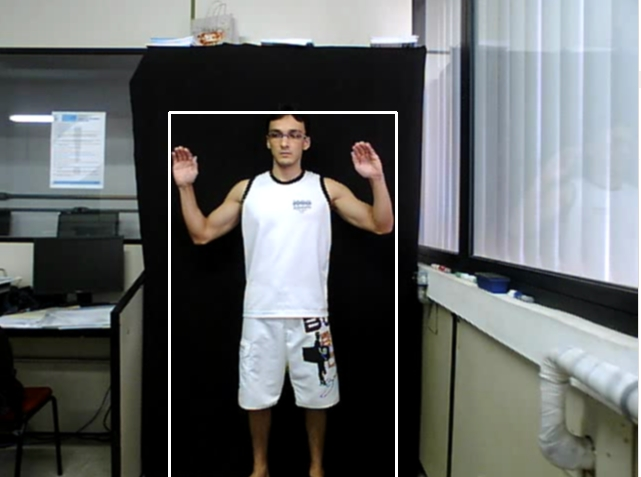
\includegraphics[width=5cm]{imagens/arms_up.jpg}}
\subfigure[img:dilate][\textit{Dilate}]{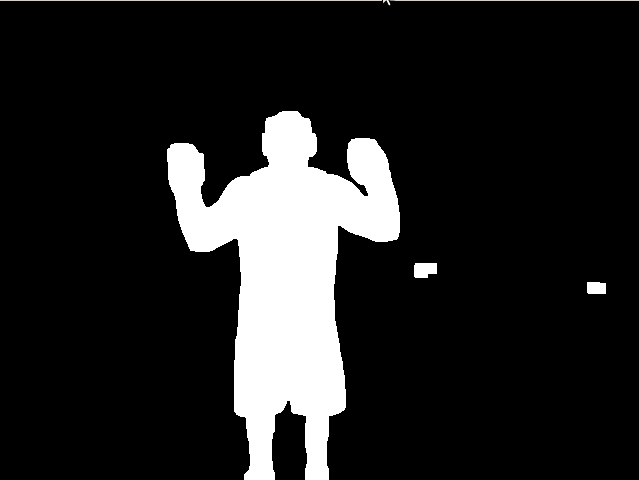
\includegraphics[width=5cm]{imagens/dilate.jpg}}
\subfigure[img:erode][\textit{Erode}]{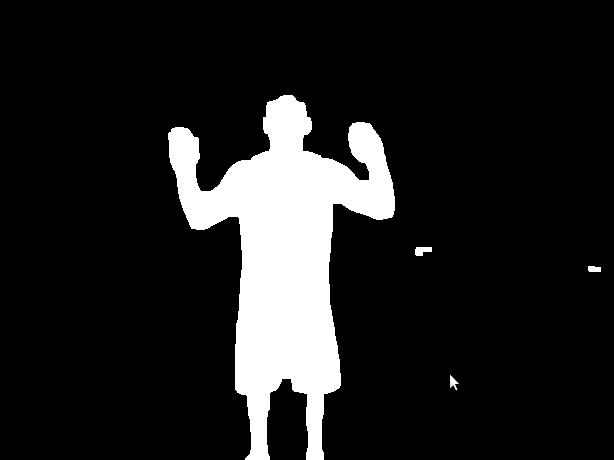
\includegraphics[width=5cm]{imagens/erode.jpg}}
\caption{Filtros de dilatação e erosão criam uma silhueta sem falhas no interior.}
\label{img:dilate_erode}
\end{figure}


\subsection{Eliminação de detecções desnecessárias}

Com a imagem binária, funções que criam contornos retangulares aos redores das formas detectadas foram usadas com o intuito de marcar os objetos de interesse. Na Figura \ref{img:maior_forma} é perceptível que mais de uma forma, como por exemplo sombras ou outras pessoas, pode ser detectada em um mesmo frame e é preciso que apenas uma forma seja levada em consideração por frame, por isso a área de cada um dos retângulos foi calculada e apenas o maior deles foi copiado para uma imagem contendo as dimensões desse retângulo, chamada de região de interesse.

\begin{figure}[!htbp]
\center
\begin{tabular}{ccc}
\subfigure{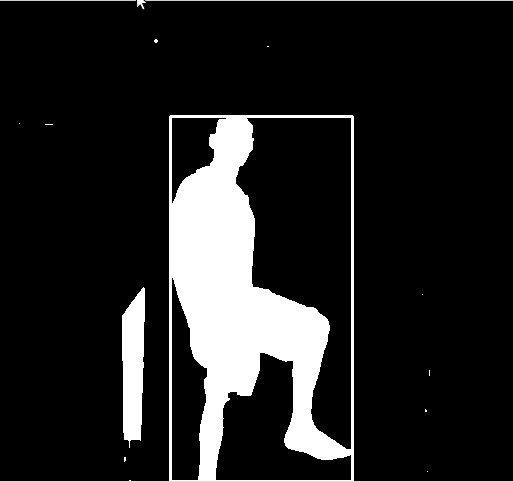
\includegraphics[scale=0.25]{imagens/maior_forma.jpg}} & \hspace{0.5cm} &
\subfigure{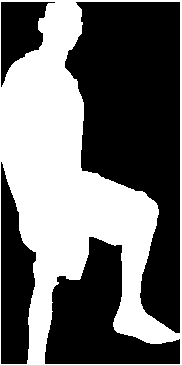
\includegraphics[scale=0.25]{imagens/maior_forma_2.jpg}} \\
Todos os contornos & & Contorno avaliado  
\end{tabular}
\caption{Quando mais de um contorno é detectados em um mesmo frame, apenas o maior é avaliado.}
\label{img:maior_forma}
\end{figure}

\section{Modelo do vetor de características}

Para formação do vetor de características \(V_f\) usou-se características de malha, por sua capacidade de descrever complexos padrões em duas dimensões com sucesso, cada imagem (\(L_f\times{A_f}\) pixels) contendo a região de interesse é dividida em segmentos de malha de tamanho \(L_s\times{A_s} \) pixels. A proporção de pixels brancos em cada malha se torna um elemento do vetor de características de acordo com,

\[V_{(i+j)} = \frac{pixelsBrancos_{(ij)}}{L_s\times{A_s}}\].

Onde $pixelsBrancos_{(ij)}$ é o número de pixels brancos no segmento $i,j$. A malha utilizada no começo do sistema tinha tamanho $3\times3$, gerando um vetor de características de tamanho 9, esse tamanho não gerou informações suficientes para diferenciar bem algumas posturas como, por exemplo, estar virado para direita ou para esquerda, gerando bastante confusão quando se estava nessas posições, aumentar a malha resolveu esse problema.
Apesar de \cite{YAMATO} terem divido os segmentos da malha em partes de $8\times8$ pixels, gerando um vetor de características de dimensão 625, esse valores pareceram excessos desnecessários, ter dobrado a altura e largura da malha no sistema  foi suficiente para os problemas de confusão nas posturas. A Figura \ref{img:malha} exibe um exemplo de malha de características de tamanho $6\times6$, utilizada no sistema final, ela gera um vetor de tamanho 36. A Tabela \ref{table:valores_malha} demonstra exemplo de valores dessas características no caso de uma malha $ 3\times{3}$ .

A biblioteca SciPy foi usada durante esse procedimento. SciPy é uma biblioteca de Open Source de ferramentas científicas para Python, ela depende da Biblioteca NumPy, que é uma biblioteca para linguagem Python que permite trabalhar com vetores e matrizes de uma forma comparável e com uma sintaxe semelhante ao software proprietário Matlab, mas com muito mais eficiência e com toda a expressividade da linguagem. SciPy reúne uma variedade de módulos para estatística, transformadas de Fourier, álgebra linear, processamento de sinais e imagens, etc.

\begin{figure}[!htbp]
  \center
  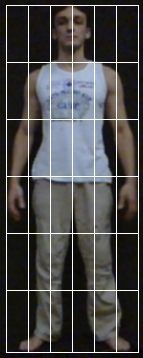
\includegraphics[scale=0.40]{imagens/malha.jpg}
  \caption{Uma malha de características de tamanho $6\times6$.}
  \label{img:malha}
\end{figure}

\begin{table}[!htbp]
\caption{Exemplos de valores de uma malha de características, 1.0 significa que o segmento da malha é todo branco e 0.0 significa que o segmento é todo preto.}
\label{table:valores_malha}
\centering
\begin{tabular}{p{4.5cm} | p{4.5cm} | p{4.5cm}}
\toprule
\small{0.27971014492753621} & \small{0.85797101449275359} & \small{0.36935817805383026} \\ \midrule
\small{0.65051759834368528} & \small{0.99109730848861288} & \small{0.74824016563147} \\ \midrule
\small{0.33830227743271224} & \small{0.44761904761904764} & \small{0.59565217391304348}\\
\bottomrule
\end{tabular}
\end{table}

\subsection{Modelo de reconhecimento de padrões}

Para o processo de reconhecimento de padrões, o método de clusterização por k-means \cite{Patter-Recognition-M-Bishop} foi utilizado. O algoritmo recebe como entrada o número de clusters \(K\) e a matriz de todos os vetores de características do treino e como saída gera os vetores de características que representam os centros desses clusters. Um vetor \(V\) pertence ao cluster \(C\) se ele está mais perto do centro de \(C\) do que quaisquer outros centros dos outros clusters. Se \(V\) for agrupado ao cluster \(C\), dizemos que o cluster \(C\) é o centro dominante de \(V\).

O algoritmo k-means realiza varias iterações para convergir para um mínimo local, em função das distâncias entre cada vetor e os centros de todos os clusters. Em geral, a convergência pode ser relativamente lenta se número de vetores e número $K$ for grande, mas neste caso o número $K$ é pequeno e o número de vetores é relativamente pequeno, por tanto será rápida a convergência. Uma boa escolha dos centros iniciais é fundamental neste método para se obter resultados eficientes. Neste caso, é escolhido como centros iniciais um conjunto de imagens representativas de cada gesto, por tanto seus respectivos vetores de características são considerados como centros iniciais. Isso garante um resultado confiável do processo de clusterização. Uma vez definidos os $K$ centros, se atribue cada vetor de características ao cluster para o qual a distância entre esse vetor e o centro desse cluster é menor que a de todos os outros clusters. Uma vez concluída a distribuição dos vetores característicos em diferentes clusters, é calculado o novo centro de cada cluster como a média aritmética de seus elementos. Se existir alguma variação entre os centros novos e os anteriores, os novos centros passam a ser os $K$ centros para uma nova iteração de clusterização, ignorando os anteriores. Esse processo é realizado enquanto houver alguma variação entre os respectivos centros, caso contrário acontece a convergência. O conjunto de $K$ centros da convergência são os vetores dominantes, que representam a os vetores característicos de seus respectivos clusters \cite{Liu}.

Todos os próximos vetores de características serão classificados de acordo com o número do cluster (também chamado de índice centróide ou índice do centro mais próximo) ao qual ele foi agrupado. Assim, por exemplo, na fase de treino, os $N_j$ vetores que pertencem ao cluster $C_j$ se identificam com o índice $j$. Na fase de reconhecimento, qualquer vetor característico da imagem em análise será testado com todos os clusters por proximidade. O índice do cluster mais próximo será atribuído como índice do vetor para ser classificado pelo modelo HMM correspondente.

O algoritmo de quantização, neste caso usando o algoritmo k-means, tenta minimizar a distorção, que é definido como a soma do quadrado das distâncias entre cada vetor de características e seu centro dominante e retorna um conjunto de índice de centros, um para cada vetor de características, esses índices serão utilizados como símbolos para as HMMs. Exemplo, para $K$ clusters, o índice das imagens que correspondem aos clusters $C_j$ é $j$, para $j = 1, ..., K$.

Neste trabalho, cada um dos 5 gestos é representado por uma sequência de $p$ frames, portanto são em total $5p$ imagens (seus respectivos vetores característicos) que devem ser clusterizados. Considera-se 4 posturas representativas que definem eficientemente cada gesto, em consequência serão $4 \times 5 = 20$ centros e 1 postura considerada default (postura parado de frente para a câmera), que implicam a definição de 21 clusters. No processo de clusterização por k-means, os 21 centros iniciais foram especificados por concepção visual de representação da postura. No final de cada processo os centros determinados nem sempre são as definidas inicialmente e possivelmente não exista uma imagem associada ao centro, devido ao fato de que em cada iteração do k-means os novos centros são determinados como a média aritmética dos elementos dos clusters.

Na Figura \ref{img:centros_clusters} se exibem as imagens centros iniciais das posturas de cada gesto. A Tabela \ref{table:codebook} exibe a estrutura do codebook, onde a posição 0 é usada para o cluster que representa a imagem parado virado de frente para câmera, os índices de 1 a 4 são escolhidos para a seqûencia de posturas que definem o gesto de dar um passo para a direita, os índices de 5 a 8 as posturas escolhidas para definir o gesto de dar um passo para a esquerda, 9 a 12 o gesto de levantar o braço direito, 14 a 16 levantar o braço esquerdo e 17 a 20 para representar o gesto de levantar ambos os braços. Dessa forma um total de 21 índices foram definidos.

A Figura \ref{img:agrupamentos} exibe alguns resultados de agrupamentos, onde todas as imagens à esquerda da seta nas figuras retornam um mesmo símbolo, o índice do centro do cluster ao qual elas foram agrupadas, representado pelo número exibido a direita das setas nas figuras, as imagens a direita da seta foram utilizadas para terem seu vetores de características extraídos para representar o centro inicial dos respectivos clusters.

\begin{table}[!htbp]
\caption{Estrutura do Codebook.}
\label{table:codebook}
\centering
\begin{tabular}{p{4.5cm} | p{6.5cm}}
\toprule
\textbf{Índice/Símbolo} & \textbf{Codeword} \\
\midrule[1pt]
0 & Parado virado de frente para câmera \\ \midrule
1 & Passo para direita 1 \\ \midrule
2 & Passo para direita 2 \\ \midrule
3 & Passo para direita 3 \\ \midrule
4 & Passo para direita 4 \\ \midrule
5 & Passo para esquerda 1 \\ \midrule
6 & Passo para esquerda 2 \\ \midrule
7 & Passo para esquerda 3 \\ \midrule
8 & Passo para esquerda 4 \\ \midrule
9 & Levantar braço direito 1 \\ \midrule
10 & Levantar braço direito 2 \\ \midrule
11 & Levantar braço direito 3 \\ \midrule
12 & Levantar braço direito 4 \\ \midrule
13 & Levantar braço esquerdo 1 \\ \midrule
14 & Levantar braço esquerdo 2 \\ \midrule
15 & Levantar braço esquerdo 3 \\ \midrule
16 & Levantar braço esquerdo 4 \\ \midrule
17 & Levantar ambos os braços 1 \\ \midrule
18 & Levantar ambos os braços 2 \\ \midrule
19 & Levantar ambos os braços 3 \\ \midrule
20 & Levantar ambos os braços 4 \\
\bottomrule
\end{tabular}
\end{table}

\begin{figure}[!htbp]
\center
\begin{tabular}{ccccccc}
	
\subfigure{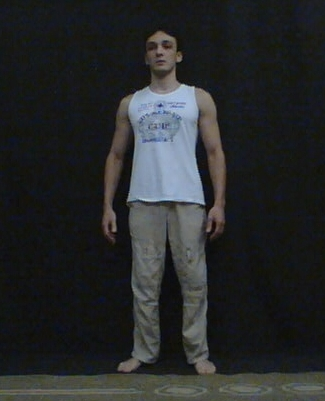
\includegraphics[scale=0.23]{imagens/codeword_parado.jpg}}
\\
(0)
\\
\subfigure{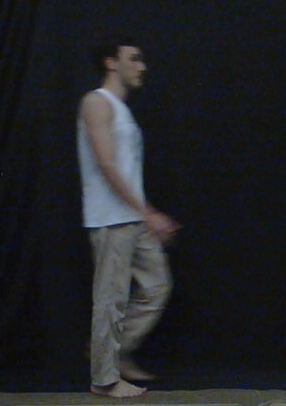
\includegraphics[scale=0.23]{imagens/codewords_passo_direita_1.jpg}} & \hspace{0.5cm} &
\subfigure{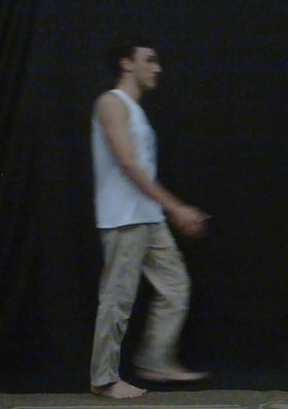
\includegraphics[scale=0.23]{imagens/codewords_passo_direita_2.jpg}} & \hspace{0.5cm} &
\subfigure{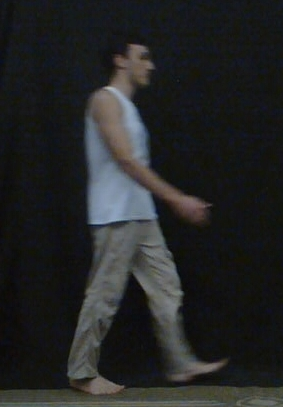
\includegraphics[scale=0.23]{imagens/codewords_passo_direita_3.jpg}} & \hspace{0.5cm} &
\subfigure{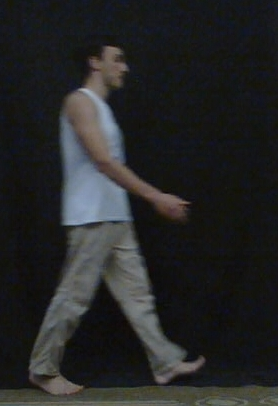
\includegraphics[scale=0.23]{imagens/codewords_passo_direita_4.jpg}}
\\
(1) & & (2) & & (3) & & (4) 
\\
\subfigure{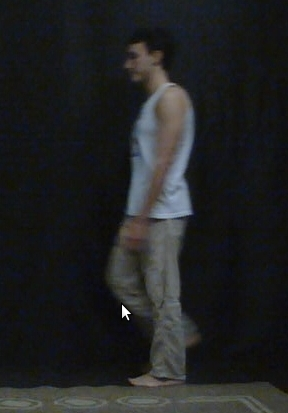
\includegraphics[scale=0.23]{imagens/codewords_passo_esquerda_1.jpg}} & &
\subfigure{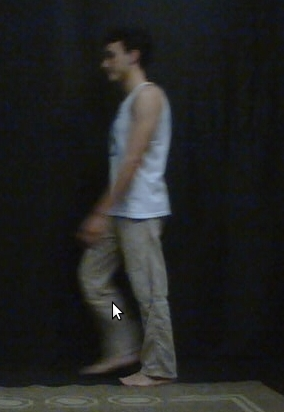
\includegraphics[scale=0.23]{imagens/codewords_passo_esquerda_2.jpg}} & &
\subfigure{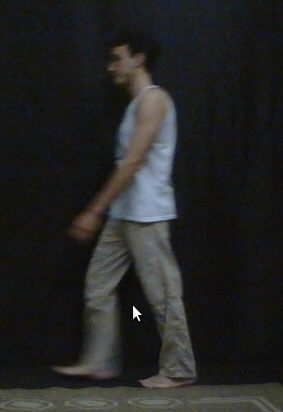
\includegraphics[scale=0.23]{imagens/codewords_passo_esquerda_3.jpg}} & &
\subfigure{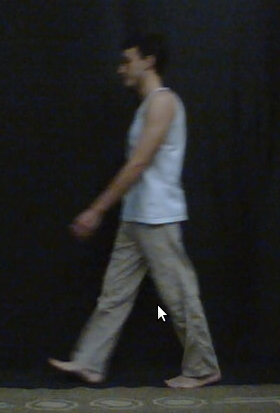
\includegraphics[scale=0.23]{imagens/codewords_passo_esquerda_4.jpg}}
\\
(5) & & (6) & & (7) & & (8) 
\\
\subfigure{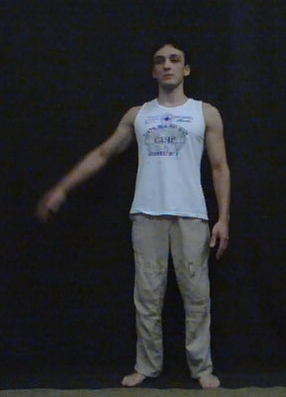
\includegraphics[scale=0.23]{imagens/codewords_braco_direito_1.jpg}} & &
\subfigure{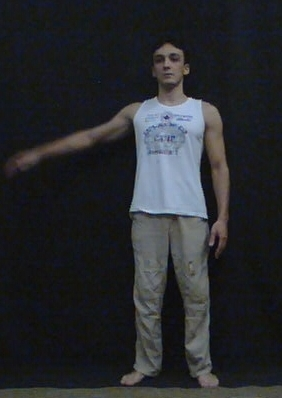
\includegraphics[scale=0.23]{imagens/codewords_braco_direito_2.jpg}} & &
\subfigure{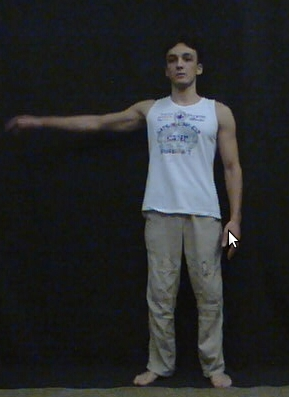
\includegraphics[scale=0.23]{imagens/codewords_braco_direito_3.jpg}} & &
\subfigure{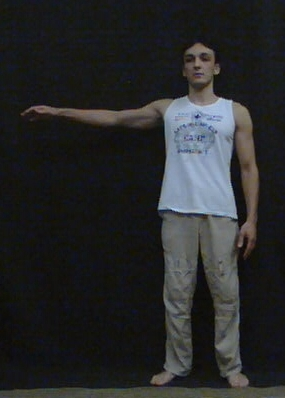
\includegraphics[scale=0.23]{imagens/codewords_braco_direito_4.jpg}}
\\
(9) & & (10) & & (11) & & (12) 
\\
\subfigure{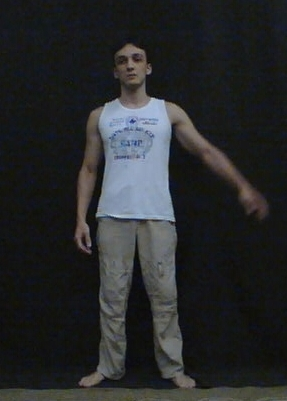
\includegraphics[scale=0.23]{imagens/codewords_braco_esquerdo_1.jpg}} & &
\subfigure{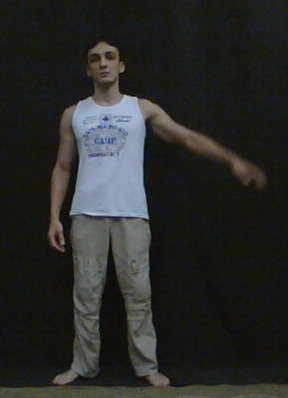
\includegraphics[scale=0.23]{imagens/codewords_braco_esquerdo_2.jpg}} & &
\subfigure{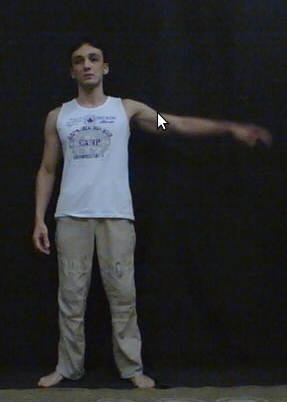
\includegraphics[scale=0.23]{imagens/codewords_braco_esquerdo_3.jpg}} & &
\subfigure{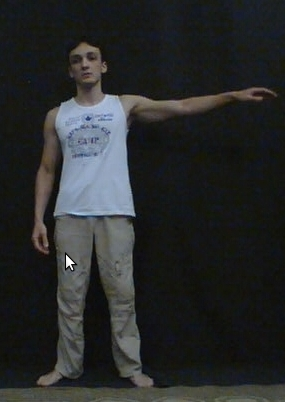
\includegraphics[scale=0.23]{imagens/codewords_braco_esquerdo_4.jpg}}
\\
(13) & & (14) & & (15) & & (16) 
\\
\subfigure{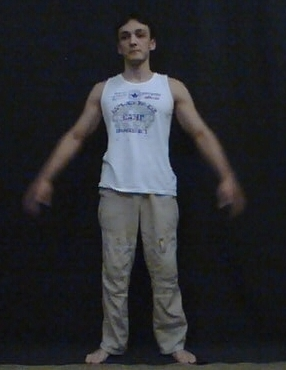
\includegraphics[scale=0.23]{imagens/codewords_2_bracos_1.jpg}} & &
\subfigure{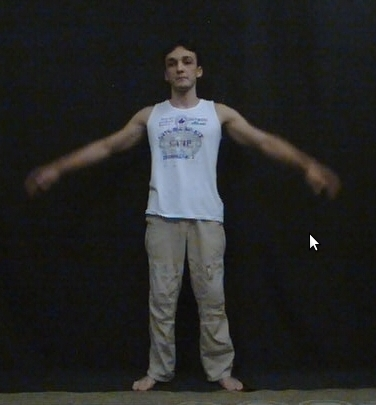
\includegraphics[scale=0.23]{imagens/codewords_2_bracos_2.jpg}} & &
\subfigure{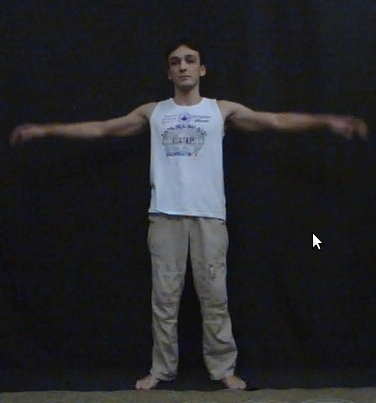
\includegraphics[scale=0.23]{imagens/codewords_2_bracos_3.jpg}} & &
\subfigure{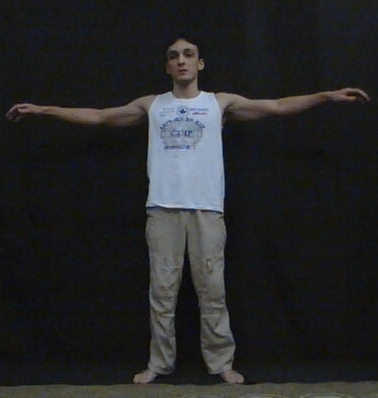
\includegraphics[scale=0.23]{imagens/codewords_2_bracos_4.jpg}}
\\
(17) & & (18) & & (19) & & (20) 

\end{tabular}
\caption{Imagens representativas dos centros dos clusters.}
\label{img:centros_clusters}
\end{figure}

\begin{figure}[!htbp]
  \center
  \subfigure{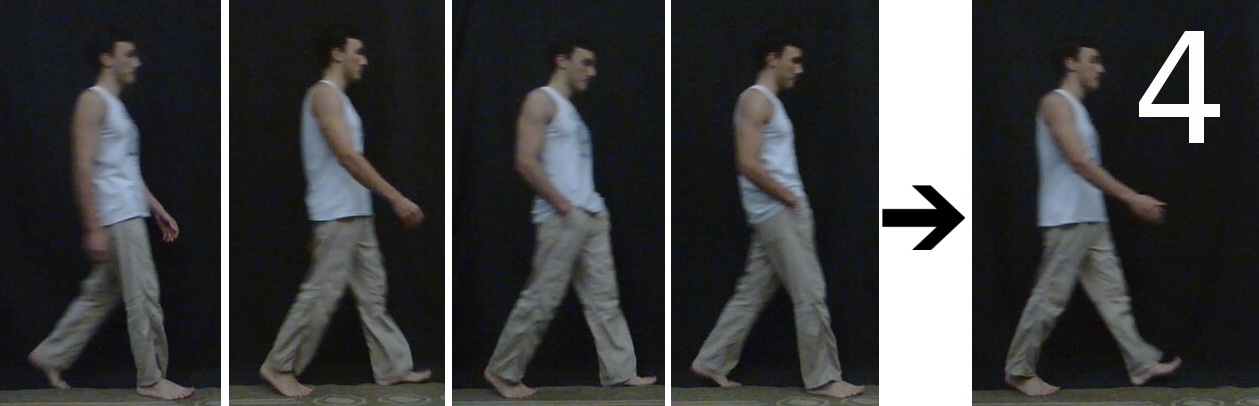
\includegraphics[width=12cm]{imagens/exemplo_vq_4.jpg}}
  \qquad
  \subfigure{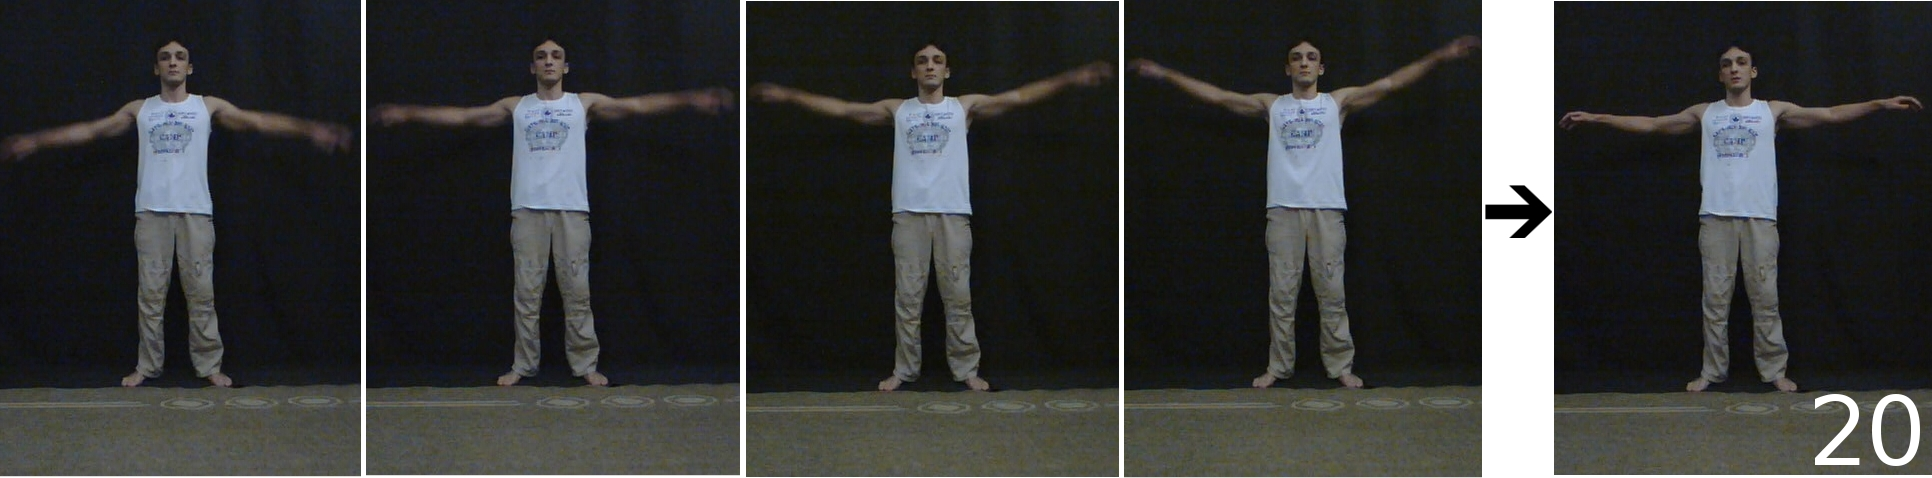
\includegraphics[width=12cm]{imagens/exemplo_vq_20.jpg}}
  \caption{As imagens a esquerda da seta foram agrupadas ao cluster de índice representado pelo número a direita da seta, todas elas serão representadas pelo símbolo correspondente a esse número nas HMMs.}
  \label{img:agrupamentos}
\end{figure}


\section{Modelagem das HMMs}

Liu et al. \cite{UnderstandingHMMTrainingForVideoGestureRecognition}, Elmezain et al. \cite{HMM-Based_Isolated_Hand_Gesture_Recognition} e Tataru et al. \cite{OnHandGesturesRecognitionUsingHiddenMarkovModels} chegaram a conclusão de que a topologia LRB (\textit{Left Right Banded}) como modelo na HMM apresenta a melhor taxa de reconhecimento. Por isso essa foi a topologia utilizada no início do sistema. A biblioteca GHMM auxiliou no processo de modelagem, treino e reconhecimento das sequências de entrada.

A topologia LRB, para o propósito deste trabalho é de quatro estados com arestas de transição entre estados adjacentes de esquerda para direita, com ciclos nos mesmos estados, tal como ilustra a Figura \ref{img:HMM_sistema}, cuja matriz de transições $A$ deve ser da seguinte forma:

\begin{equation}\label{matriz_A}
  A =
    \begin{pmatrix}
      a_{11} & 1-a_{11} & 0 & 0 \\
      0 & a_{22} & 1-a_{22} & 0 \\
      0 & 0 & a_{33} & 1-a_{33}  \\
      0 & 0 & 0 & 1
    \end{pmatrix}
\end{equation}

\begin{figure}[!htbp]
  \center
  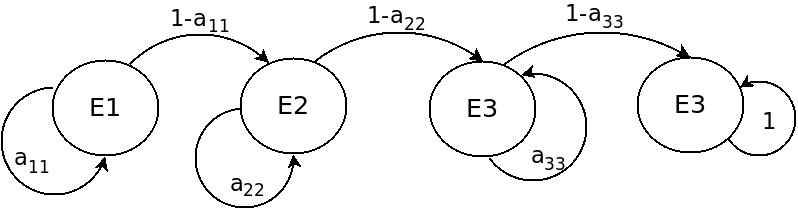
\includegraphics[scale=0.40]{imagens/HMM_sistema.jpg}
  \caption{Aplicação da matrix $A$ na topologia LRB.}
  \label{img:HMM_sistema}
\end{figure}

Durante o processo de criação da HMM $\lambda$ é necessária a inicialização do valores $\lambda(A, B, \pi)$. Segundo \cite{UnderstandingHMMTrainingForVideoGestureRecognition}, a matriz \(A\) nessa topologia é inicializada através da computação da duração \(d\) do estado de acordo com
\[d = \frac{T}{N}\], onde \(N\) é número de estados da HMM e \(T\) é o tamanho da duração do gesto. A taxa de imagens gravadas pela câmera é de 30 frames por segundo, o sistema foi projetado para a cada segundo enviar os últimos 30 símbolos para serem avaliados em cada HMM, portanto o valor de $T = 30$ nesse sistema. O número de estados que cada HMM contém é 4, devido ao fato de que cada gesto possui 4 símbolos. Essa duração segmenta a sequência de observação uniformemente; portanto cada estado possui a mesma duração, nesse caso \(d\) equivale a \( 30/4 = 7.5\), dai que \(a_{ii} = 1/d\), logo a matriz \(A\) associada à Figura \ref{img:HMM_sistema}, segundo (\ref{matriz_A}), é inicializada da seguinte forma

\[
 A =
 \begin{pmatrix}
  0.75 & 0.25 & 0 & 0 \\
  0 & 0.75 & 0.25 & 0 \\
  0 & 0 & 0.75 & 0.25  \\
  0 & 0 & 0 & 1
 \end{pmatrix}.
\]

O segundo parâmetro a ser inicializado é a matriz \(B\), os estados de uma cadeia HMM são discretos, portanto todos os elementos da matriz \(B\) podem ser inicializados com o mesmo valor para todos os estados. A matriz \(B\) será inicializada da seguinte forma 
\[B = \{b_{im}\}, \mbox{ para } b_{im} = \frac{1}{M}, \mbox{ onde } 1 \leq i \leq N, 1 \leq m \leq M; \] 
sendo \(N\) o número de estados e \(M\) a quantidade de símbolos, tal como foi estabelecido anteriormente na sessão \ref{hmm}. O terceiro parâmetro é o vetor \(\pi\), que assumirá

\[
 \pi =
 \begin{pmatrix}
  1 & 0 & 0 & 0
 \end{pmatrix},
\]
porque deve-se garantir que a HMM sempre começá pelo primeiro estado. A Figura \ref{img:HMM_antes_treino} demonstra o grafo das HMMs criadas utilizando-se os parâmetros acima.

\begin{figure}[!htbp]
  \center
  \caption{HMMs antes do processo de treino.}
  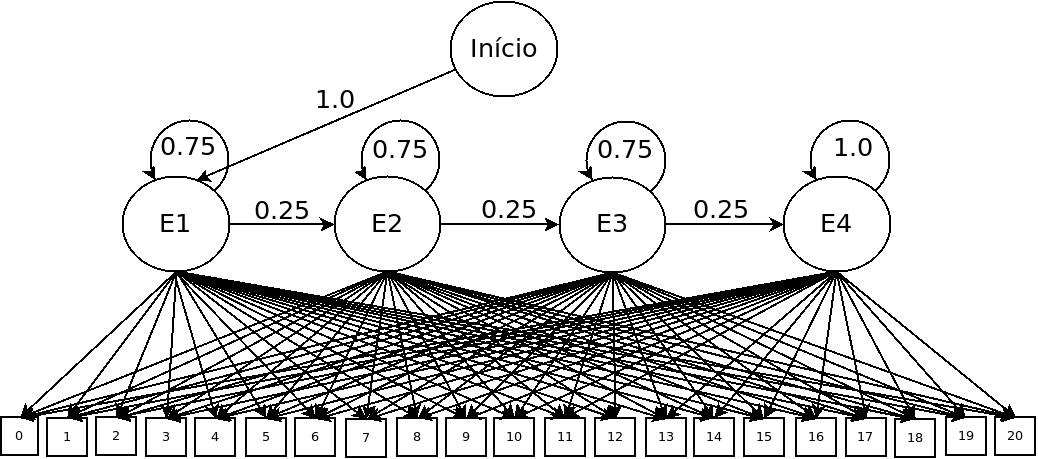
\includegraphics[scale=0.40]{imagens/HMM_antes_treino.jpg}
  \label{img:HMM_antes_treino}
\end{figure}

\subsection{Processo de treinamento}

Os símbolos de saída da quantização vetorial precisam ser armazenados em um vetor, para serem posteriormente avaliados pelo algoritmo de Viterbi. No trabalho de Elmezain et al. \cite{HMM-Based_Isolated_Hand_Gesture_Recognition}, o sistema foi projetado para reconhecer gestos com significados a partir da detecção da codeword zero. Isso significa que o vetor de símbolos começa a ser construído a partir do momento que um símbolo zero é reconhecido e o final desse vetor acontece quando outro símbolo zero é identificado.

Se fosse implementar esse modelo nesse sistema, uma postura específica para ser representada pela codeword zero haveria de ser criada e todos os meus gestos começariam e terminariam com essa postura, seria importante que essa postura também não aparecesse durante os gestos para que os mesmos não tivessem seus vetores interrompidos.

Essa postura no começo e no fim dos gestos não tornaria a interação tão natural quanto se pudéssemos implementar um sistema onde ela não fosse necessária, por esse motivo, esse sistema funciona enviando a cada segundo, todos os símbolos reconhecidos nesse tempo. Já que a câmera que foi utilizada captura trinta imagens por segundo, trinta símbolos são armazenados e enviados para o módulo de reconhecimento a cada segundo.

Seria ideal que cada um dos quatro estados da HMM retornasse apenas um dos quatro símbolo de cada gesto. Se não houvesse ruídos ou erros de distorções, em condições ideais cada segundo de vídeos produziria uma sequência parecida com, por exemplo; \[[1,1,1,1,1,1,1,1,2,2,2,2,2,2,2,3,3,3,3,3,3,3,4,4,4,4,4,4,4,4]\].
Essa sequência seria facilmente reconhecida como "passo a direita" pela classificação de uma HMM configurada para produzir a maior probabilidade desses símbolos aparecerem nessa ordem. Essa HMM ideal é representada na Figura \ref{img:HMM_1_ideal}.

\begin{figure}[!htbp]
  \center
  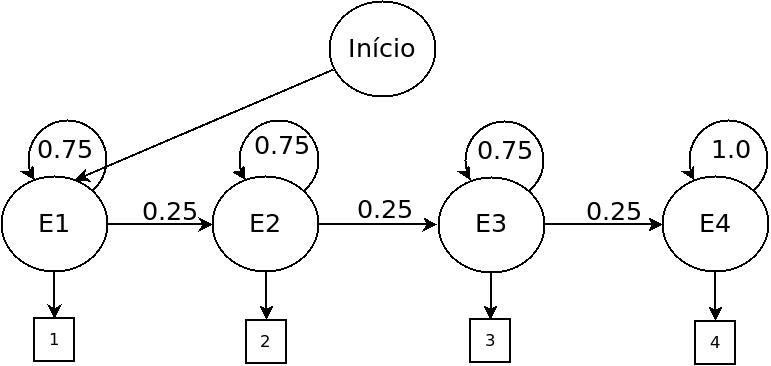
\includegraphics[scale=0.35]{imagens/HMM_1_ideal.jpg}
  \caption{Parâmetros de uma HMM configurada para reconhecer um passo a direita, se não houvesse ruído e/ou erro.}
  \label{img:HMM_1_ideal}
\end{figure}

Na realidade isso não acontece e um único símbolo errado ou com distorção maior, comprometeria todo o processo de reconhecimento. Por exemplo, de sequência para ser reconhecida pelo sistema poderia ser
\[[17, 1, 1, 1, 2, 2, 3, 3, 3, 3, 4, 4, 4, 4, 4, 4, 17, 1, 1, 1, 2, 2, 2, 3, 3, 3, 3, 4, 4, 4]\]
que se aproxima mais do gesto um "passo a direita" do que todos os outros, por conter a maior parte de símbolos associados a esse gesto, o sistema deve ser capaz de lidar com essas variações e ainda assim fazer identificações correta.

É inviável tentar estimar os melhores valores (ótimos) para as parâmetros \((A, B, \pi)\). Na verdade, o problema de treinar um grafo desta característica com valores exatos é um problema difícil, por tanto se recorre a métodos de aproximação como Baum-welch o qual o resultado é uma convergência local. Nesse sentido, para treino de HMM o algoritmo de Baum-welch é utilizado recebendo como entrada as sequências de símbolos extraídas de cada um dos quatro vídeos gravados de cada um dos gestos. Para cada um dos 5 gestos é gerado um modelo HMM a partir do modelo inicial proposto e considerando que todos os estados possuem saídas para todos os símbolos, tal como mostrado na Figura \ref{img:HMM_antes_treino}. Os modelos gerados são $\lambda_1, \lambda_2, \lambda_3, \lambda_4$ e $\lambda_5$, os quais são mostrados pelas figuras \ref{img:HMM_5_apos_treino}, \ref{img:HMM_4_apos_treino}, \ref{img:HMM_3_apos_treino}, \ref{img:HMM_2_apos_treino} e \ref{img:HMM_1_apos_treino}, respectivamente.

\begin{figure}[!htbp]
  \center
  \caption{Parâmetros de uma HMM treinada com os vídeos do gesto levantar ambos os braços.}
  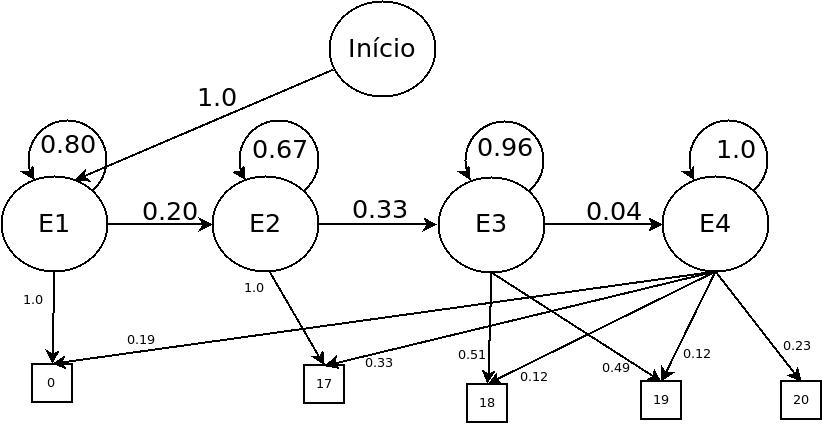
\includegraphics[scale=0.35]{imagens/HMM_5_apos_treino.jpg}
  \label{img:HMM_5_apos_treino}
\end{figure}

\begin{figure}[!htbp]
  \center
  \caption{Parâmetros de uma HMM treinada com os vídeos do gesto levantar o braço esquerdo.}
  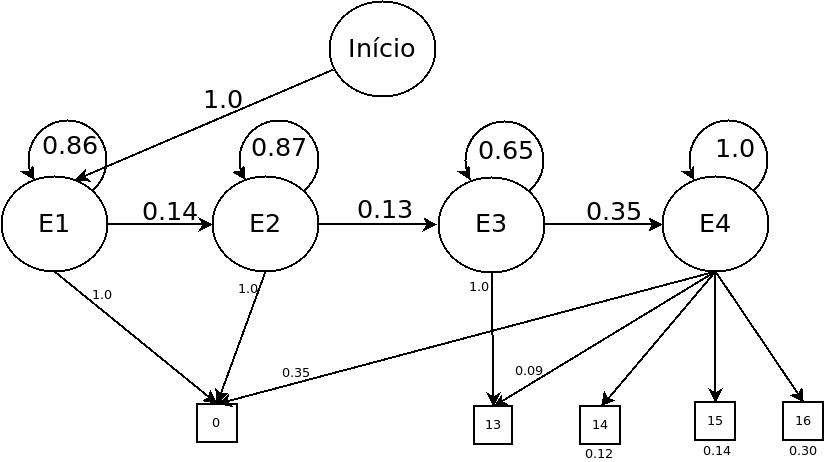
\includegraphics[scale=0.35]{imagens/HMM_4_apos_treino.jpg}
  \label{img:HMM_4_apos_treino}
\end{figure}

\begin{figure}[!htbp]
  \center
  \caption{Parâmetros de uma HMM treinada com os vídeos do gesto levantar o braço direito.}
  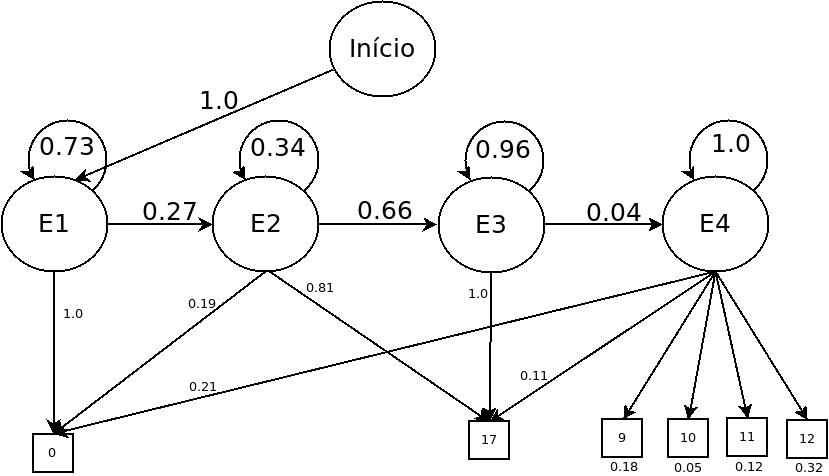
\includegraphics[scale=0.35]{imagens/HMM_3_apos_treino.jpg}
  \label{img:HMM_3_apos_treino}
\end{figure}

\begin{figure}[!htbp]
  \center
  \caption{Parâmetros de uma HMM treinada com os vídeos de passos a direita.}
  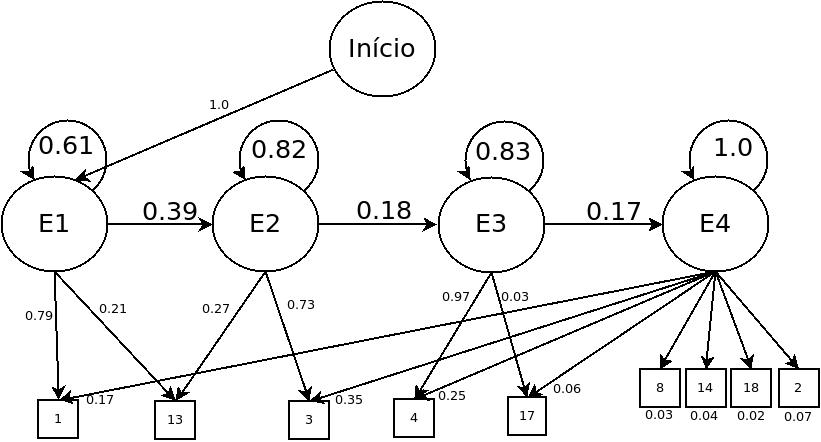
\includegraphics[scale=0.35]{imagens/HMM_1_apos_treino.jpg}
  \label{img:HMM_1_apos_treino}
\end{figure}

\begin{figure}[!htbp]
  \center
  \caption{Parâmetros de uma HMM treinada com os vídeos de passos a esquerda.}
  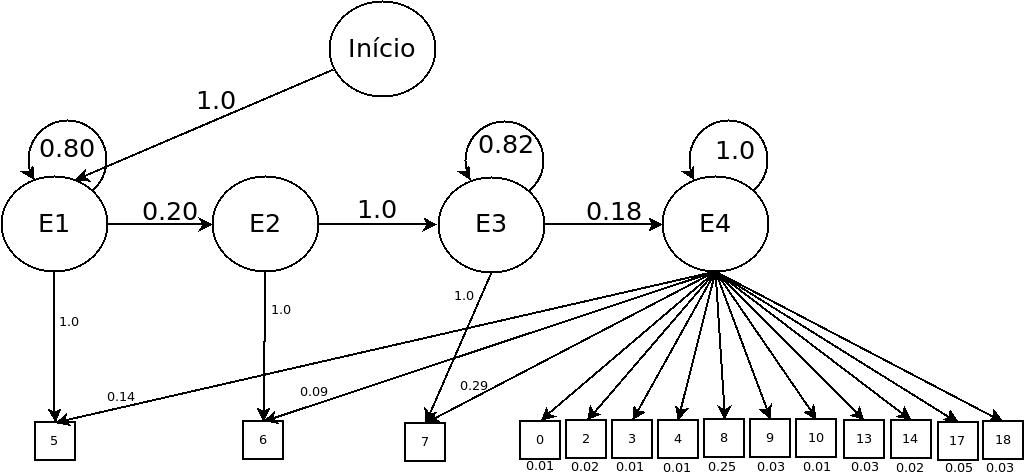
\includegraphics[scale=0.35]{imagens/HMM_2_apos_treino.jpg}
  \label{img:HMM_2_apos_treino}
\end{figure}


\subsection{Modelo de identificação}

A cada segundo de vídeo os últimos trinta símbolos são armazenados em um vetor e avaliados pelo algoritmo de Viterbi em cada uma das cinco HMMs, o retorno é a sequência do caminho mais provável e a probabilidade desse caminho em cada um dos cinco modelos respectivamente. Um outro vetor armazena todas essas probabilidades para avaliação posterior da maior delas e consequentemente o gesto mais provável. Depois dessa avaliação o vetor de símbolos é esvaziado para ser preenchido novamente no próximo segundo.

Na maioria dos reconhecimentos, a sequência recebida só retornava probabilidade em uma das HMMs, todas as outras tinham chance nula de ser a HMM responsável pela sequência de símbolos de entrada. Para ilustrar essa situação, observe um exemplo de vetor de símbolos que foi armazenado em um dos segundo de uma sequência de vídeo onde o usuário está caminhando para a direita, que gerou a seguinte sequência de símbolos observáveis: \[[1, 1, 1, 1, 2, 3, 3, 3, 3, 3, 8, 4, 4, 4, 4, 4, 17, 17, 1, 1, 1, 2, 3, 3, 3, 3, 8, 4, 4, 4].\] A Tabela \ref{table:viterbi_1} exibe as probabilidades calculadas através dos caminhos mais prováveis, em todas as HMMs, dessa sequência de símbolos acontecer.

Se observarmos os grafos das HMMs treinadas, verificaremos que a probabilidade é nula na segunda HMM, porque ela tem não tem chance alguma de retornar o símbolo 1, enquanto a terceira, quarta e quinta também tem probabilidade nula de retornar os símbolos 2, 3 e 4.

Quando a todos os modelos retornam probabilidade nula, nenhum gesto é reconhecido naquele segundo e nenhum comando é enviado ao avatar no ambiente virtual, portanto ele fica executando uma animação default, enquanto aguarda um reconhecimento bem sucedido.

\begin{table}[!htbp]
\caption{Tabela de exemplo de probabilidades avaliadas pelo algoritmo de Viterbi.}
\label{table:viterbi_1}
\centering
\begin{tabular}{p{5.5cm} | p{5.5cm}}
\toprule
\textbf{HMM} & \textbf{Probabilidade} \\
\midrule[1pt]
1 - Passo para direita & -63.091143841560843 \\ \midrule
2 - Passo para esquerda & Nenhuma \\ \midrule
3 - Levantar braço direito & Nenhuma \\ \midrule
4 - Levantar braço esquerdo & Nenhuma \\ \midrule
5 - Levantar ambos os braços & Nenhuma \\
\bottomrule
\end{tabular}
\end{table}

